\begin{surferPage}[八階曲面]{霍穆托夫八次曲面}
乍一看上去,霍穆托夫(Chmutov)八次曲面$\text{Chm}_{d}, \ d=8,$具有明顯的對稱性。這也能從它的定義方程看出來:\[\text{Chm}_{d}\colon T_d(x) + T_d(y) + T_d(z) + 1 = 0,\]其中$T_d$是所謂的切比雪夫多項式(Tchebychev polynomial,左圖)。曲線$T_8(x)+T_8(y)=0$是右圖。
     \begin{center}
      \begin{tabular}{c@{\quad}c}
        \begin{tabular}{c}
          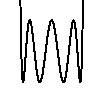
\includegraphics[height=1.75cm]{Tcheb_008.pdf}
        \end{tabular}
        &
        \begin{tabular}{c}
          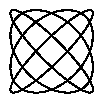
\includegraphics[height=1.75cm]{Tcheb_2d_008.pdf}
        \end{tabular}
      \end{tabular}
    \end{center}
    \vspace{-0.3cm}
從這些圖到交互式圖中的曲面形狀也就幾步之遙。

這些方程由霍穆托夫在上世紀80年代給出。對大多數$d$, 由他們構造的$\mu(d)$成為了當時的世界紀錄。
上世紀90年代,霍穆托夫更新了他自己的紀錄。2005年,松加·布萊斯克(Sonja Breske)、奧利弗·萊布斯(Oliver Labs)與杜克·范·斯特芬(Duco van Straten)用這個構造產生了只有實奇異點的實曲面。
\end{surferPage}
